% !TeX root = ../main.tex

\section{Kotlin Multiplatform Mobile}
Kotlin Multiplatform Mobile\footnote{\url{https://kotlinlang.org/lp/mobile/}} (KMM) è un SDK\footnote{Software Development Kit} per lo sviluppo di app iOS e Android basato sul concetto di condivisione della logica applicativa mantenendo lo sviluppo nativo della UX/UI\footnote{User Experience/User Interface}. Fornisce i benefici sia dello sviluppo cross-platform che dello sviluppo nativo:
\begin{itemize}
    \item risparmio di tempo e risorse derivanti dalla condivisione del codice (cross-platform),
    \item alte performance (nativo),
    \item accesso diretto alle funzionalità dei dispositivi hardware senza overhead (nativo).
\end{itemize}
Con il rilascio di Kotlin 1.4 (Agosto 2020), KMM è passato dalla fase "\textit{Experimental}" alla fase "\textit{Alpha}" permettendone l'utilizzo in produzione. Tra le tantissime aziende che hanno già adottato KMM in produzione per lo sviluppo delle proprie applicazioni mobile è possibile trovare nomi rilevanti come Netflix, VMware e Philips\footnote{\url{https://kotlinlang.org/lp/mobile/case-studies/}}.\\
In base al risultato dell'indagine di mercato svolta nei primi due quadrimestri del 2021\cite{kmm2}, le parti di codice condiviso nelle applicazioni sviluppate con KMM sono:
\begin{itemize}
    \item 85\% Networking
    \item 75\% Data Storage
    \item 70\% Utility (Logging, Analytics, ...)
    \item $\sim$60\% Algoritmi/Computazione
    \item $\sim$55\% State Management
    \item $\sim$50\% Presenters/Controllers/ViewModel
\end{itemize}
Nonostante lo scopo di KMM sia quello di condividere solamente la logica applicativa, dalla indagine è risultato che il 38\% dei partecipanti vorrebbe poter condividere anche la parte relativa alla UX/UI.

\subsection{Architettura}
\begin{figure}[H]
\centering
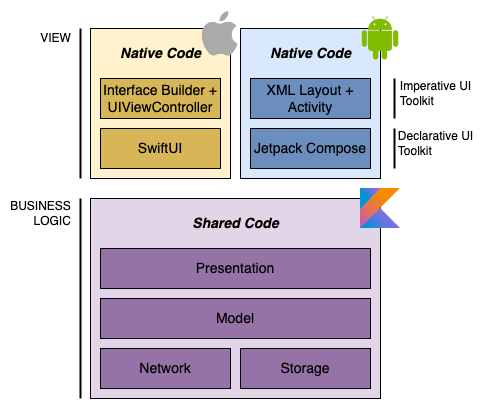
\includegraphics[width=0.7\textwidth]{img/tesi-8-kmm.drawio.png}
\caption{Architettura Kotlin Multiplatform Mobile}
\end{figure}

\subsection{KMM Plugin}